\chapter{Current Work}
\noindent \underline{\textbf{Note:}} Some models discussed in this section have certain functions and function blocks that are derivative of existing custom Simulink$^{\circledR}$ libraries and code excerpts from GitHub repositories. In such a case, the relevant sources have been duly cited wherever appropriate.

\paragraph{}
This section discusses several optimization models for predictive control for self-driving cars. The first sub-section briefly covers re-implementations of some existing models in Simulink$^{\circledR}$ in order to explore the characteristics of an MPC controller and the effect of design parameters on model response. The second sub-section illustrates a Python implementation of an MPC controller for obstacle avoidance.

\paragraph{}
The discussions in this section are mostly limited to the results and performance of the models, and code excerpts are provided wherever necessary. A detailed code implementation of all the simulations discussed below can be found in the following GitHub repository: \href{https://github.com/omprabhu31/mpc_self_driving_cars}{\texttt{omprabhu31/mpc-self-driving-cars}}.

\section{Re-implementation of existing models}

\subsection{Basic MPC controller model for lateral and steering control}
\paragraph{}
This section discusses the implementation of a basic MPC controller that has been designed to control an autonomous vehicle steering system. The driving task consists of performing a smooth overtake maneuver without having a very high rate of change of the steering angle. Note that the only feedback to the MPC controller is the plant output (i.e., the lateral position and yaw angle). The vehicle states (i.e., velocity, heading and position coordinates) are not part of the feedback loop. As a result, it is not possible for this type of MPC controller to handle varying velocity input. The control loop for this scenario has been illustrated in Figure 4.1.

\paragraph{}
The simulation discussed above has been implemented by consulting a web-based Mathworks tutorial$^{\text{[4]}}$ available on the Internet. The `reference signal' and `plant' simulation blocks have been used directly from a Simulink$^{\circledR}$ library called \texttt{Meldas\_library}. These blocks provide functions for transformation of the controller output (i.e., the steering angle) to the plant output using standard vehicle dynamics equations.

\begin{figure}[H]\label{fig4.1}
\centering 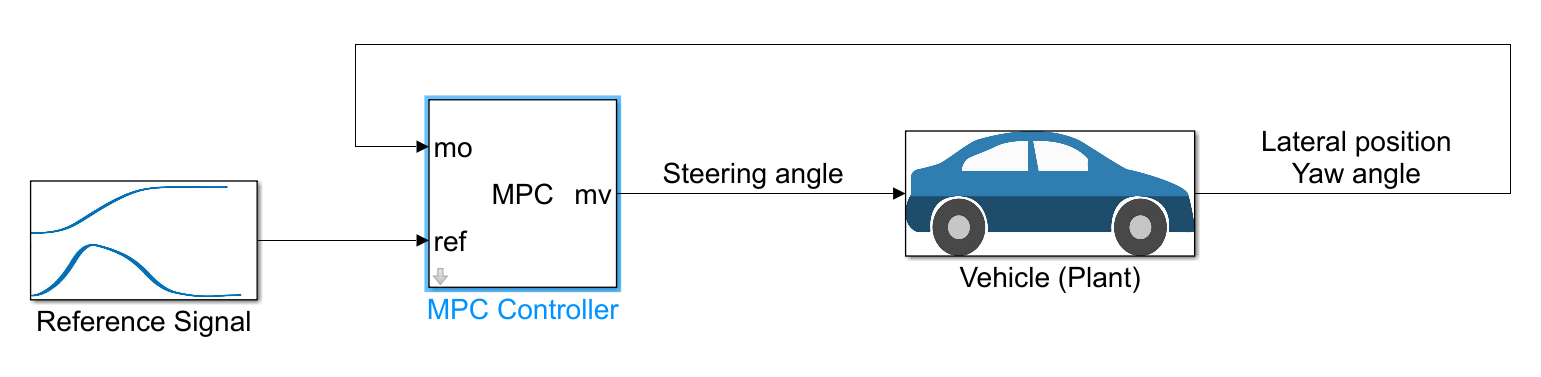
\includegraphics[scale=0.4]{Images/basic_mpc_model.png}
\caption{Basic MPC Control Loopn for Autonomous Vehicle Control}
\end{figure}

\begin{figure}[H]\label{fig4.2}
\centering 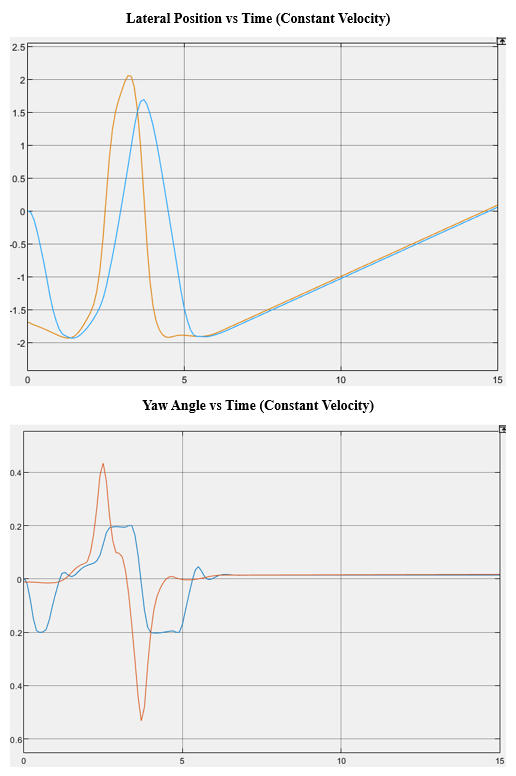
\includegraphics[scale=1.1]{Images/basic_mpc_constant_response.png}
\caption{Basic MPC Controller Response to Constant Velocity Input}
\end{figure}
\paragraph{}
Figures 4.2 and 4.3 illustrate the response of this control system to a fixed velocity input and a sinusoidal velocity input respectively. As observed, the controller has near perfect tracking for a constant velocity input. If the desired velocity or prediction horizon is increased, the controller displays a somewhat tardy response, but still provides an acceptable response for a basic overtake maneuver. 

\paragraph{}
However, for a time-varying velocity input, the controller response is not ideal. The control output (i.e., steering angle) and plant output both diverge with time. To tackle this problem involving varying velocity, we need to implement an adaptive MPC controller which allows for feedback of vehicle states back to the controller.

\begin{figure}[H]\label{fig4.3}
\centering 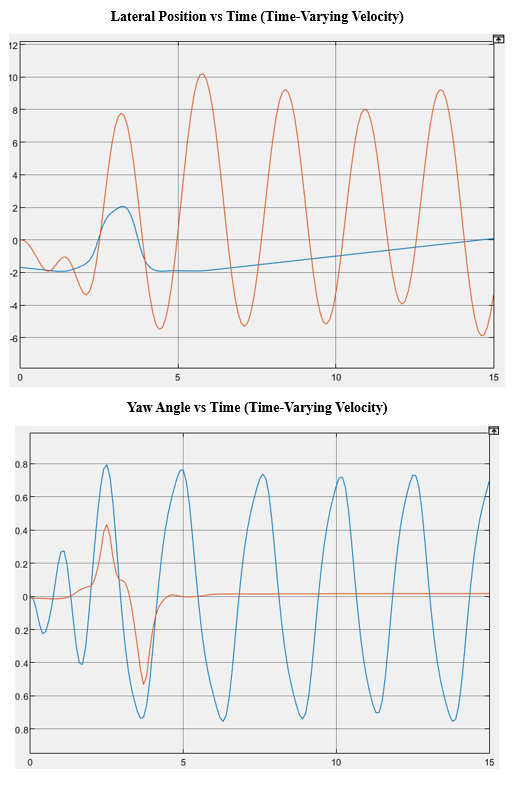
\includegraphics[scale=1.1]{Images/basic_mpc_varying_response.png}
\caption{Basic MPC Controller Response to Varying Velocity Input}
\end{figure}

\subsection{Adaptive MPC controller model for lateral and steering control}
\paragraph{}
This section discusses the implementation of an adaptive MPC controller that has been designed to control an autonomous vehicle steering system. The driving task still remains that of performing an overtake maneuver. The control loop for this scenario has been illustrated in Figure 4.4. Note that, unlike the basic MPC controller, we also introduce the vehicle states as feedback to the controller. Hence, it is possible for us to implement control of vehicle velocity as well as steering angle by updating the vehicle dynamics model at each time step.

\paragraph{}
The above simulation has been implemented by consulting a web-based Mathworks tutorial$^{\text{[5]}}$ available on the Internet. The `reference signal' and `plant' simulation blocks have been used directly from a Simulink$^{\circledR}$ library called \texttt{Meldas\_library}. These blocks provide functions for transformation of the controller output (i.e., the steering angle) to the plant output using standard vehicle dynamics equations.

\paragraph{}
The \texttt{tf\_fn} block carries out a transformation from the vehicle states to the state-space matrices of the vehicle model. It makes use of standard vehicle dynamics equations involving the vehicle parameters, states and controller sample time to compute a discrete-time plant model.

\begin{figure}[H]\label{fig4.4}
\centering 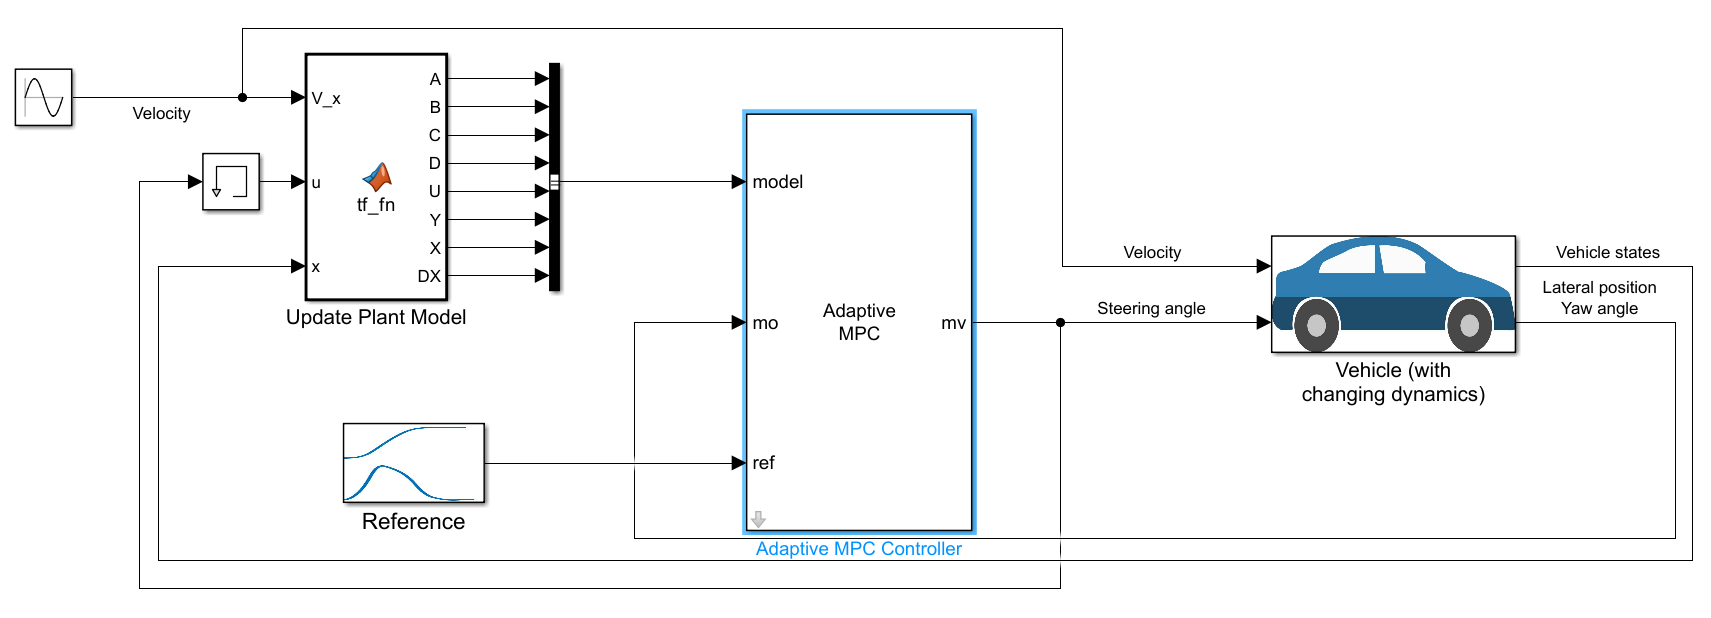
\includegraphics[width=\textwidth]{Images/adaptive_mpc_model.png}
\caption{Adaptive MPC Control Loop}
\end{figure}

\paragraph{}
As expected, the output response in case of a constant velocity is identical to that of the basic MPC controller (refer to Figure 4.2 for output response plots). Figure 4.5 illustrates the response of the adaptive MPC control system to a time-varying velocity input. For simulation purposes, we have employed a sample-based sinusoidal velocity input, but the controller performs just as well for any other varying velocity function. While the traditional MPC controller discussed in the previous section failed to track a time-varying velocity input, the adaptive MPC model is able to satisfactorily track a sinusoidal velocity input. 

\paragraph{}
This example illustrates the effectiveness of an adaptive MPC controller to take into account changing plant dynamics as part of the controller feedback loop. Note that the output response for the yaw angle does deviate slightly compared to the reference signal - this is because we have employed constrained on the maximum and minimum values of the yaw angle as well as yaw rate in order to avoid sudden jerks.

\begin{figure}[H]\label{fig4.5}
\centering 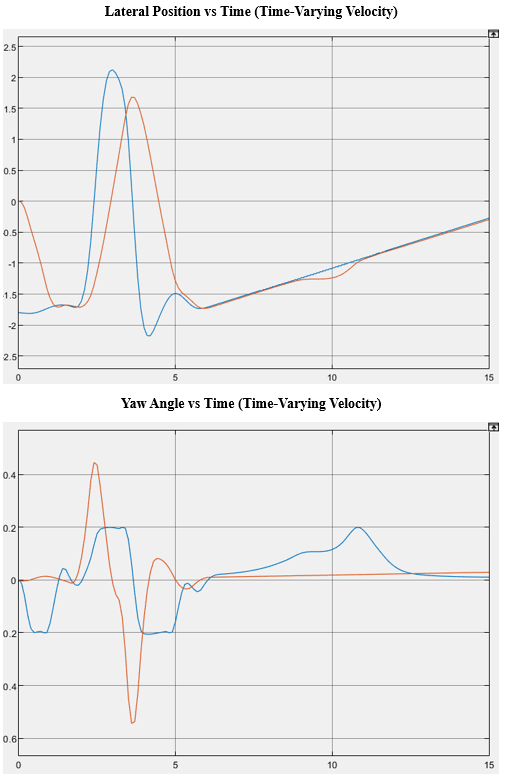
\includegraphics[scale=1.1]{Images/adaptive_mpc_varying_response.png}
\caption{Adaptive MPC Controller Response to Sinusoidal Velocity Input}
\end{figure}

\subsection{MPC controller model for path tracking across a racetrack}
\paragraph{}
This section discusses a the implementation of an adaptive MPC controller that has been designed to traverse a given racetrack. Because performing steering maneuvers along sharp turns is one of the major challenges faced in autonomous steering control, we select a track comprising two circular loops placed adjacent to each other, mimicking a figure-eight shape. The driving task is to traverse the path with reasonable accuracy.
\newpage

\paragraph{}
The simulation of a vehicle traversing a figure-eight loop involves the following steps:
\begin{enumerate}[label = (\arabic*), itemsep=-0.3em]
    \item defining the reference points for the figure-eight track by specifying the radius of the circular loops and step size of angles to be traversed
    \item calculating the reference pose and curvature vectors using the linearized distance vectors
    \item transforming the vehicle parameters and state variables (velocity, torque, etc) to compute the state-space matrices for the vehicle dynamics model
    \item compute the curvature function to maintain the vehicle along the curved path
\end{enumerate}

\paragraph{}
The control for this driving scenario is illustrated in Figure 4.6. Note that this model employs the use of 3-degree of freedom vehicle dynamics instead of the simple 2-degree of freedom bicycle model discussed earlier in Section 2. At the current stage, this lies outside the scope of the project and hence, the code for the same been adapted from an online Mathworks repository$^{\text{[6]}}$. This includes the parts of the simulation involving the powertrain \& driveline system and the transformation functions for mapping vehicle states to the 3-DOF model parameters. 

\begin{figure}[H]\label{fig4.6}
\centering 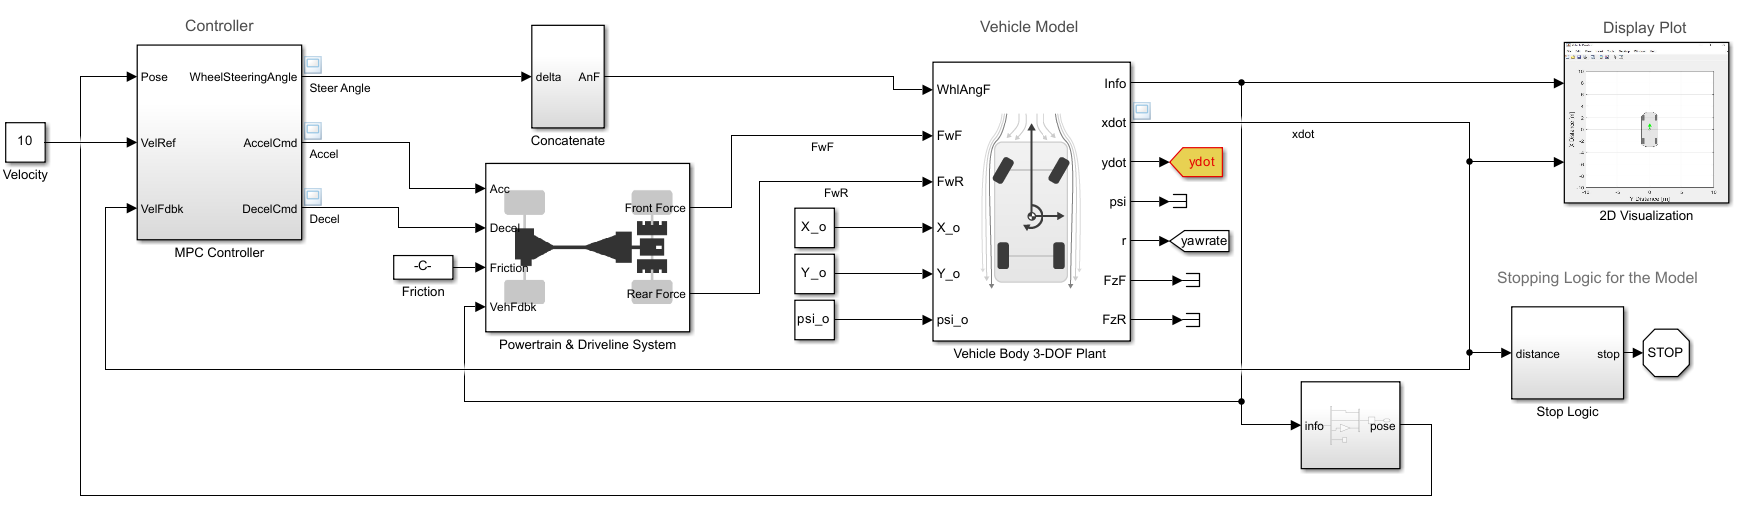
\includegraphics[width=\textwidth]{Images/figure_eight_model.png}
\caption{Control Loop for Path Tracking Along a Racetrack}
\end{figure}

\paragraph{}
Figures 4.7 and 4.8 illustrate the response of the above control system to various operating conditions (red plot represents reference trajectory, black plot represents model response). As observed, the performance of the MPC controller is near perfect for tracking the reference trajectory at reasonably low values of desired vehicle velocity. As we increase the desired velocity, the controller displays a tardy response and the trajectory tracking output is significantly worse. This is an expected behaviour, since the task of turning corners or performing roundabout maneuvers is significantly more difficult at higher speeds even with current manual control vehicles. As is seen in Figure 4.8, the model struggles to keep up with the reference trajectory at high velocities. In fact, setting the vehicle speed to 30 m/s causes the MPC algorithm to reach an infeasible solution while tracking the loop.

\paragraph{}
Note that the model discussed above only allows for a fixed vehicle speed. However, in real life, we rarely wish to perform sharp turning maneuvers at fixed speeds. To counter this problem, we can instead employ an adaptive MPC controller in order to include the vehicle states as part of the feedback control loop. This potential improvement to the model is discussed in greater detail in Section 5 of the report.

\begin{figure}[H]\label{fig4.7}
\centering 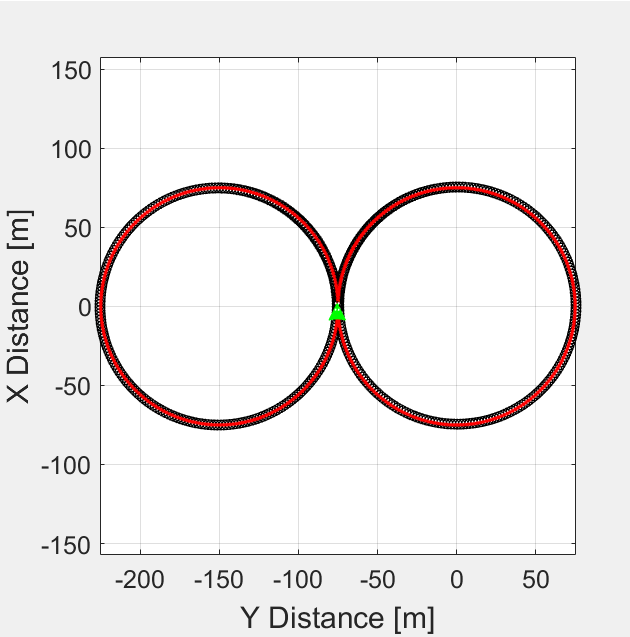
\includegraphics[scale=0.8]{Images/low_velocity_tracking_response.png}
\caption{Vehicle Path Tracking Response for Low Reference Velocity (10 m/s)}
\end{figure}

\begin{figure}[H]\label{fig4.8}
\centering 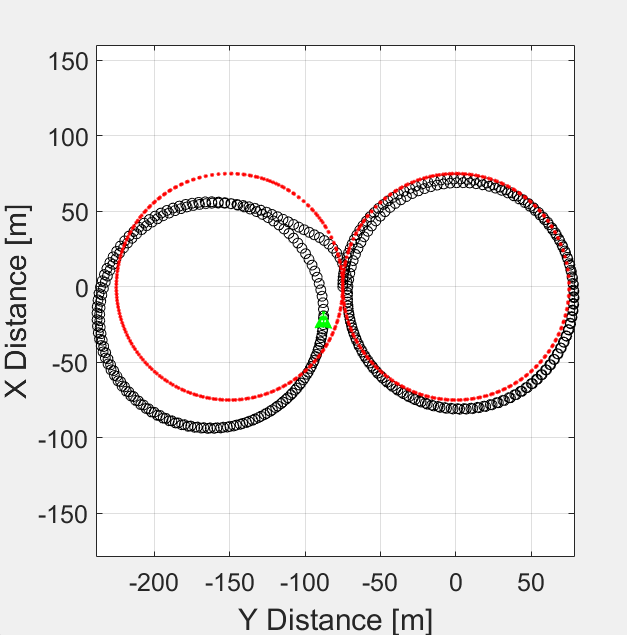
\includegraphics[scale=0.8]{Images/high_velocity_tracking_response.png}
\caption{Vehicle Path Tracking Response for High Reference Velocity (25 m/s)}
\end{figure}

\subsection{MPC controller model for generation of obstacle constraints}
\paragraph{}
This section discusses the implementation of an adaptive MPC controller for dynamic generation of obstacle constraints. The simulation initially starts out with an empty set of constraints (barring the constraints on velocity and steering angle) and updates them upon detection of an obstacle based on several parameters such as obstacle \& safe zone dimensions, detection distance and distance of the vehicle from the obstacle. The driving task is straightforward - the vehicle must avoid the obstacle (and preferably also avoid entering the safe zone) by switching to the adjacent lane and then coming back to it's original lane. Without loss of generality, we assume that the vehicle always shifts into the left lane to avoid the obstacle. The control loop for this driving scenario is illustrated in Figure 4.9.

\paragraph{}
Some aspects of the code for this simulation have been adapted from a web-based Mathwork's tutorial$^{\text{[7]}}$, including code for plotting the obstacle avoidance maneuver and relationships between some of the simulation blocks used to store vehicle states and for passing the generated constraints to the adaptive MPC controller. 

\begin{figure}[H]\label{fig4.9}
\centering 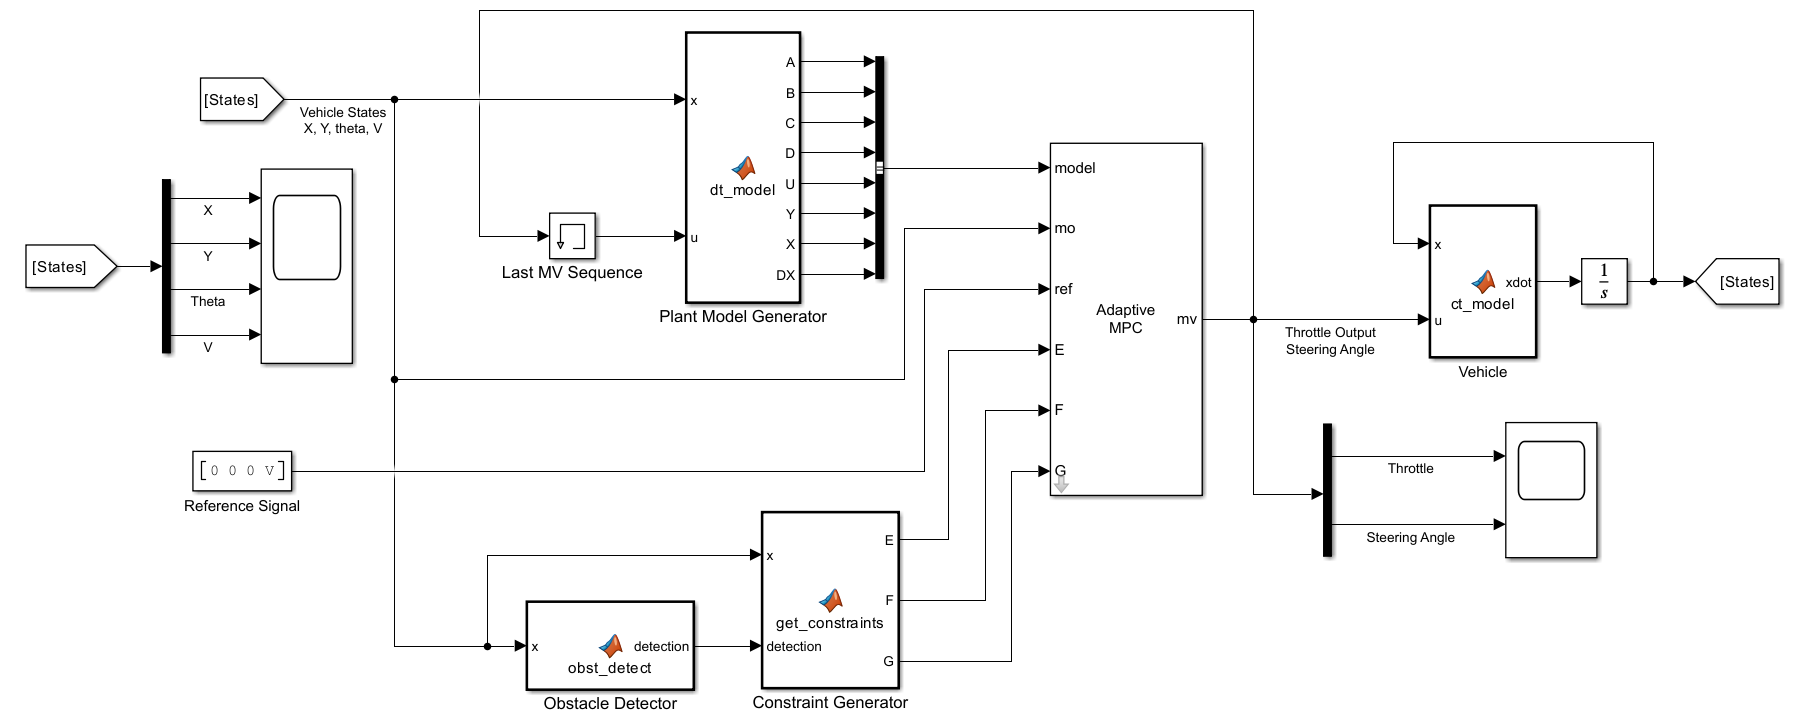
\includegraphics[width=\textwidth]{Images/obstacle_avoidance_model.png}
\caption{Adaptive MPC Control Loop for Obstacle Avoidance}
\end{figure}

\paragraph{}
Apart from the velocity and steering angle constraints, we dynamically compute the obstacle constraints at each time step. This is done as follows:
\begin{enumerate}[label = (\arabic*), itemsep=-0.3em]
    \item As the vehicle travels along its path, the distance between the vehicle and the obstacle decreases until it hits the obstacle detection distance
    \item Once the vehicle detects the obstacle, it computes a safe zone around the obstacle
    \item For every time step, we impose the following constraints:
    \begin{enumerate}[label = (\roman*), itemsep=-0.3em]
        \item vehicle must not collide with the obstacle (hard constraint)
        \item vehicle must not enter the safe zone as far as possible (soft constraint)
        \item draw a hypothetical line passing through the nearest corner of the safe zone and the current position - the vehicle must not cross the region to the right of this line (soft constraint)
    \end{enumerate}
\end{enumerate}

\paragraph{}
Depending on the vehicle's starting velocity, it may or may not end up violating the soft constraints. For example, if the starting velocity of the vehicle is very high, it will be unable to decelerate in time - this is because we have also imposed constraints on the rate of acceleration to avoid sudden jerks in the response. In such a case, the vehicle may violate the safe constraints and cross into the obstacle's safe zone and/or the partition defined by the third constraint.

\begin{figure}[H]\label{fig4.10}
\centering 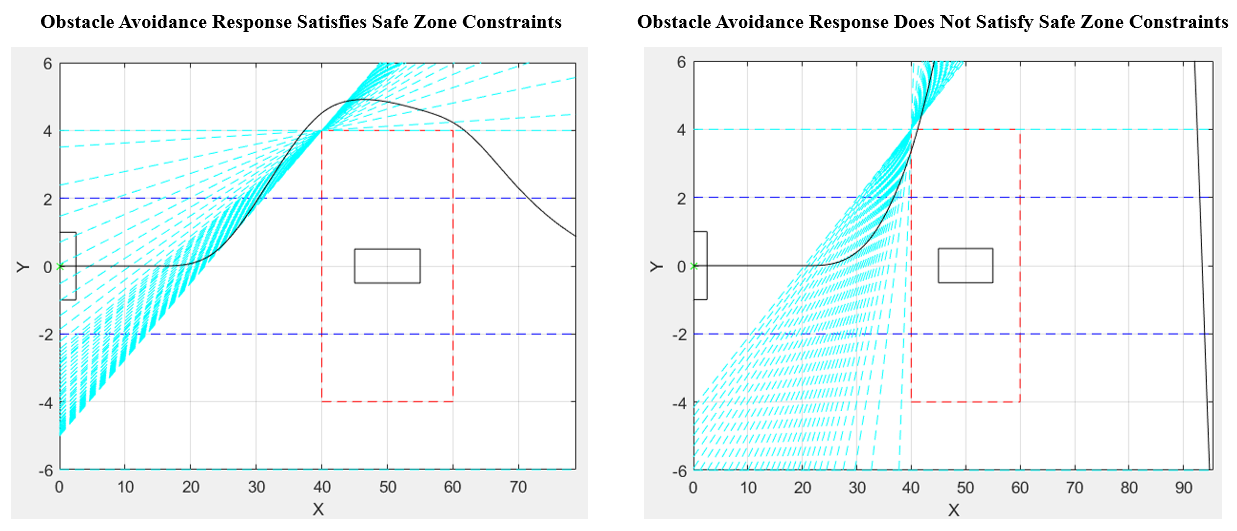
\includegraphics[width=\textwidth]{Images/satisfies_and_violate_safe_zone.png}
\caption{Variation of Obstacle Avoidance Response with Initial Velocity}
\end{figure}

\paragraph{}
The prediction horizon also has a considerable effect on the output response. In general, the longer the prediction horizon, the smoother the output response. This is because the optimization is solved for a larger number of future time steps. As illustrated in Figure 4.11, the simulation with the smaller prediction horizon displays a much tighter output response. It also crosses into the safe zone while returning back into its original lane. On the other hand, the simulation with the larger prediction horizon provides a much smoother and generally safer obstacle avoidance maneuver. However, a large prediction horizon may cause computational difficulties in some cases.

\begin{figure}[H]\label{fig4.11}
\centering 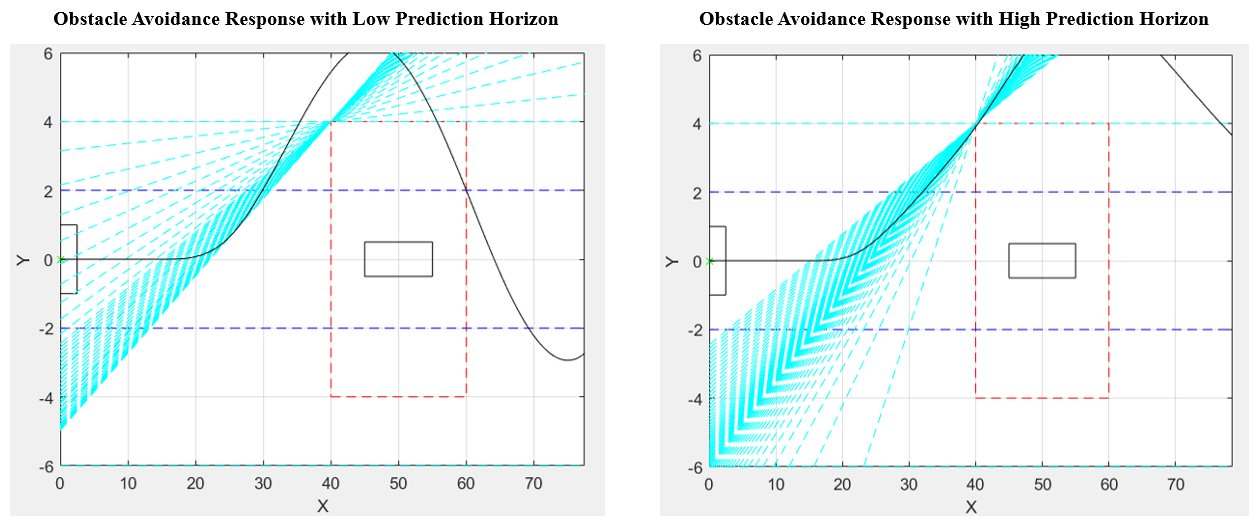
\includegraphics[width=\textwidth]{Images/high_vs_low_prediction_horizon.png}
\caption{Obstacle Avoidance Response for Low and High Prediction Horizons}
\end{figure}

\section{Model predictive controller for trajectory tracking and obstacle avoidance}
\paragraph{}
This section discusses a model that performs the driving tasks of tracking a reference trajectory, similar to the model outlined in section 4.1.3, as well as avoids obstacles in its path, much like the model discussed in section 4.1.4. This model has been implemented in Python using the \texttt{ipopt} library for solving the optimization problem. The model comprises several files which perform the following functions:
\begin{enumerate}[label = (\roman*), itemsep=-0.3em]
    \item \texttt{main.py}: the main model file, which loads the map \& simulation environment, sets up and solves the MPC problem, and plots the vehicle's position at each time step
    \item \texttt{MPC.py}: defines a class to store the characteristics of the MPC controller, get data regarding time-varying parameters (waypoints and lateral position errors), and generate obstacle constraints
    \item \texttt{model.py}: defines a class for the simple bicycle model and defines functions for model setup and getting the current waypoint from the reference path
    \item \texttt{reference\_path.py}: (adapted from an online GitHub repository$^{\text{[8]}}$) defines the \texttt{ReferencePath} class accessed in \texttt{main.py} and \texttt{model.py}
    \item \texttt{simulator.py}: (adapted from an online GitHub repository$^{\text{[8]}}$) defines the \texttt{Simulator} class used in \texttt{main.py}
    \item \texttt{map.py}: (adapted from an online GitHub repository$^{\text{[8]}}$) defines the \texttt{Map} and \texttt{Obstacle} classes use in \texttt{main.py}
    \item \texttt{globals.py}: defines global variables (distance covered by the vehicle and the prediction horizon) referenced by multiple files in the simulation
\end{enumerate}

\paragraph{}
Figure 4.12 illustrates the output response of the model at a particular time step. With each time step, the vehicle position is updated on the plot. The obstacle constraints and optimal control outputs are predicted by the MPC algorithm and updated on plot as well. As expected, the model results in a response that tracks the reference trajectory with a high accuracy, except for certain parts where it is forced to go off-track due to the presence of obstacles.

\begin{figure}[H]\label{fig4.12}
\centering 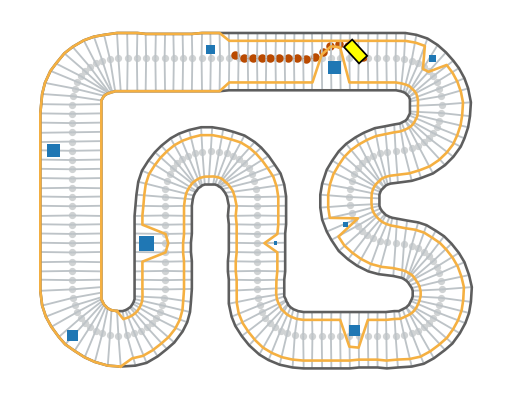
\includegraphics[scale=1]{Images/simulation_screenshot.png}
\caption{Trajectory Tracking and Obstacle Avoidance Response of MPC Controller (Python Simulation)}
\end{figure}